As stated in the introduction, metasurfaces are 2D materials with some sub-wavelength structure. Their properties are determined by the geometry of this structure which is usually a simple shape, like a rectangle or oval, on a periodic grid. The shape is called metaatom and in the case of plasmonic metasurfaces it is made of metal.
With the $S$-matrix calculus and SASA we can fully describe stacks of homogeneous isotropic materials but we still have no understanding of what happens when we add a metasurface to a stack. To build some intuition for how a specific metasurface will affect the transmission spectrum of a stack, we will need a little more theory on optics in materials. As stated before, all optical properties of a material a captured by the $\vb D$ and $\vb H$ fields and in our context
\begin{equation} \label{eq:bg:D}
    \vb D = 
    \epsilon_0 \, \vb E + \vb P =
    \epsilon_0\, \underbrace{\qty(1 + \chi)}_{
         := \epsilon
    }\, \vb E
\end{equation}
so the $\vb D$ field is determined by the $\vb E$ field and dielectric function $\epsilon$. In the following sections we will discuss which materials have which kind of dielectric functions and how we can use these to gain some understanding of the optical mechanisms in a metasurface.

\paragraph{Dielectric Function}~\\
In the simplest model we can describe electrons in a material as an ensemble of harmonic oscillators

\begin{equation} \label{eq:bg:lorentz}
    m \ddot{\vb x} + m \gamma \dot{\vb x} + m \omega_0^2 \vb x = -e \vb E,
\end{equation}

with the displacement $\vb x$, electron mass $m$, electron charge $e$, dampening factor $\gamma$ and resonance frequency $\omega_0$.
In this model the macroscopic polarization $\vb P$ is directly caused by this displacement $\vb x$ through
\begin{equation} \label{eq:bg:P}
    \vb P = - \rho e \vb x,
\end{equation}

where $\rho$ is the density of electrons.
If we assume a harmonic time dependency $\vb E(t) = \vb E_0 e^{i \omega t}$ equation \eqref{eq:bg:lorentz} is solved by 
\begin{equation}
    \vb x(t) = \frac{e}{m(\omega^2 + i \gamma \omega - \omega_0^2)} \vb E(t)
\end{equation}

and using equation \eqref{eq:bg:D} and \eqref{eq:bg:P} this results in the $\vb D$ field
\begin{equation}
    \vb D = 
    \epsilon_0 \underbrace{ 
    \qty(1 - \frac{f}{\omega^2 + i \gamma \omega - \omega_0^2})
    }_{
        =\epsilon
    }
    \vb E,
\end{equation}

where $f = \rho e^2 / \epsilon_0 m$ is the oscillator strength.
In a real material there are always multiple resonance frequencies $\omega_m$ but in good approximation these do not influence each other and the total dielectric function can be obtained simply by summing over all $m$ \cite{FOMO}
\begin{equation}
    \epsilon(\omega) := 
    \epsilon'(\omega) + i \epsilon''(\omega) = 
    1 + \sum_m \frac{f_m}{\omega_m^2 - \omega_0^2 - i \gamma \omega}
\end{equation}

\begin{figure}[H]
    \floatbox[{
    \capbeside
    \thisfloatsetup{capbesideposition={right,top}}}]{figure}[\FBwidth]
    {\caption{
        Example plots for the real and imaginary part of the refractive index 
        $n = \eta + i\kappa$
        as calculated by the multiple resonance Lorentz model.
        \cite{FOMO}
    }
    \label{fig:bg:lorentz}}
    {
\includegraphics[width=0.5\textwidth]{bg_lorentz}}
\end{figure}

\begin{figure}[H]
    \centering
    \begin{subfigure}{.5\textwidth}
        \centering
        
\includegraphics[width=.8\linewidth]{bg_dielectric}
        \caption{}
        \label{fig:bg:dielectric}
    \end{subfigure}%
    \begin{subfigure}{.5\textwidth}
        \centering
        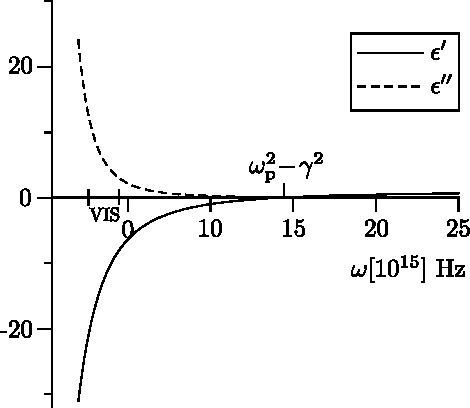
\includegraphics[width=.8\linewidth]{bg_metal}
        \caption{}
        \label{fig:bg:metal}
    \end{subfigure}
    \caption{Imaginary and real part of the dielectric function 
    $\epsilon = \epsilon' + i \epsilon''$
    for dielectrics (a) and metals (b) in the visible spectrum.
    \cite{FOMO}}
    \label{fig:bg:dm}
    \end{figure}

In section \ref{sec:s_mats} we have already discussed how the dielectric function is related to the complex refractive index by
\begin{equation}
    \epsilon = n^2 = (\eta + i \kappa)^2
\end{equation}

and this relationship is used to generate figure \ref{fig:bg:lorentz}. We observe high $\kappa$, so high absorption, at the resonance frequencies in the from of Lorentz peaks. Between resonance frequencies generally 
$\partial \eta / \partial \omega > 0$.
This is called normal dispersion and explains, for example, why red light is diffracted stronger than blue light.
Figure \ref{fig:bg:lorentz} is just a general example. To understand metasurfaces we need to discuss how the resonance frequencies are distributed in real materials.
\\

\indent
Dielectrics in the visible spectrum are well described by two resonance frequencies. One in the IR and one in the UV range. That means in the visible spectrum we have a vanishing imaginary part $\epsilon''$ of the dielectric function and normal dispersion as seen in figure \ref{fig:bg:dielectric}. 
Metals on the other hand are characterized by their high availability in free charges, thereby eliminating the restoring force ($\omega_0 = 0$) and reducing the dielectric function to 
\begin{equation}
    \epsilon(\omega) = 1 - \frac{\omega_\s p^2}{\omega^2 + i \gamma \omega}\, ,
\end{equation}

with the plasma frequency 
$\omega_\s p^2 = f = \rho e^2 / \epsilon_0 m$.
This results in a large negative $\epsilon'$ and a positive $\epsilon''$ as seen in figure \ref{fig:bg:metal}. The negative $\epsilon'$ is responsible for the reflection of visible light at metallic surfaces.

\paragraph{Surface Plasmon Polaritons}~\\
Finally, we can discuss the mechanism behind the optical properties of plasmonic metasurfaces. These work by allowing the excitation of a special electromagnetic wave at a metal dielectric interface called Surface Plasmon Polariton (SPP). This wave is confined to and travels along the interface until its energy is lost via absorption or scattering. That means it enables some photons to be absorbed by coupling into the interface. At which wavelengths this conversion occurs depends on the metasurface geometry and can thus be tailored for a specific optical target.

\begin{figure}[H]
    \centering
    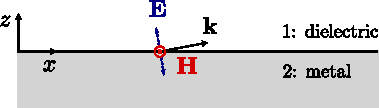
\includegraphics[width=.6\linewidth]{bg_md_interface}
    \caption{Metal dielectric interface with light in a TM mode.}
    \label{fig:bg:md_inderface}
\end{figure}

Suppose the described wave exists as a TM mode, as can be seen in figure \ref{fig:bg:md_inderface}, and has the form 

\begin{equation}
\begin{aligned}
    E_x &= E_0 e^{i k_x x - k_z z} \\
    E_z &= E_0 \frac{k_x}{k_z} e^{i k_x x - k_z z}\\
    H_y &= H_0 e^{i k_x x - k_z z}
\end{aligned}
\end{equation}

That is, propagating along the $x$ axis and evanescently decaying along the $z$ axis. This wave does indeed satisfy Maxwell's equation and the continuity conditions discussed in section \ref{sec:s_mats} if and only if \cite{Maier2007}

\begin{equation} \label{eq:bg:con1}
    \frac{\epsilon_1}{k_{z1}} = - \frac{\epsilon_2}{k_{z2}} 
\end{equation}

and

\begin{equation} \label{eq:bg:con2}
    k_x^2 + k_{zn}^2 = \epsilon_n \frac{\omega^2}{c^2}
    \qq{for}
    n = 1,2.
\end{equation}

Equation \eqref{eq:bg:con1} explains why SPP's are only possible at metal dielectric interfaces because $\epsilon'_1$ and $\epsilon'_2$ need to have different signs and this is fulfilled precisely for metals and dielectrics as can be seen in figure \ref{fig:bg:dm}. If we solve equation \eqref{eq:bg:con1} and \eqref{eq:bg:con2}, we can obtain the dispersion relation for SPP's

\begin{equation}
    k_x = \frac{\omega}{c}
    \qty(\frac{\epsilon_1 \epsilon_2}{\epsilon_1 + \epsilon_2})^{1/2}.
\end{equation}

This dispersion relation is shown in figure \ref{fig:bg:dispersion}. For small wave vectors SPP's behave like light but then they start to have increasingly lower energy $E = \hbar \omega$ compared to a free photon at the same momentum $\vb p = \hbar \vb k$. However, for a conversion Photon $\rightarrow$ SPP both energy and momentum have to be conserved.
Thus excitation of SPP's is not possible at a simple smooth metallic surface, but rather the wave vector of an incident photon has to be matched to that of an SPP of the same energy by the surface geometry.
\\

\indent
To summarize, photons can couple into a plasmonic metasurface by exiting a special electromagnetic wave called Surface Plasmon Polariton confined to the interface. The exact wavelength at which this conversion is possible depends on the metaatom geometry and can thus be easily tuned to create different optical behaviors.

\begin{figure}[H]
    \floatbox[{
    \capbeside
    \thisfloatsetup{capbesideposition={right,top}}}]{figure}[\FBwidth]
    {\caption{
        Dispersion relation for light and Surface Plasmon Polaritons in air (grey) and silica (black). Frequency and wave vector are normalized to the plasma frequency $\omega_\s p$ \cite{Maier2007}.
    }
    \label{fig:bg:dispersion}}
    {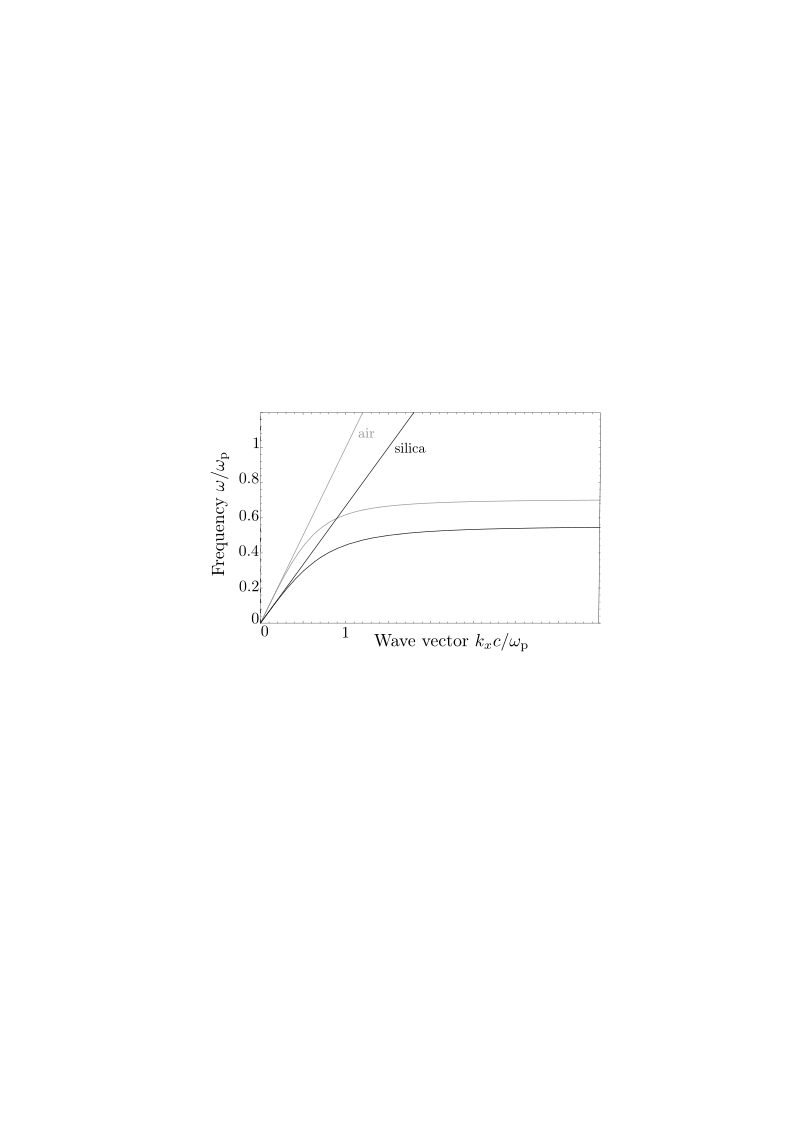
\includegraphics[width=0.55\textwidth]{bg_dispersion}}
\end{figure}